% Options for packages loaded elsewhere
\PassOptionsToPackage{unicode}{hyperref}
\PassOptionsToPackage{hyphens}{url}
%
\documentclass[
]{article}
\usepackage{amsmath,amssymb}
\usepackage{iftex}
\ifPDFTeX
  \usepackage[T1]{fontenc}
  \usepackage[utf8]{inputenc}
  \usepackage{textcomp} % provide euro and other symbols
\else % if luatex or xetex
  \usepackage{unicode-math} % this also loads fontspec
  \defaultfontfeatures{Scale=MatchLowercase}
  \defaultfontfeatures[\rmfamily]{Ligatures=TeX,Scale=1}
\fi
\usepackage{lmodern}
\ifPDFTeX\else
  % xetex/luatex font selection
\fi
% Use upquote if available, for straight quotes in verbatim environments
\IfFileExists{upquote.sty}{\usepackage{upquote}}{}
\IfFileExists{microtype.sty}{% use microtype if available
  \usepackage[]{microtype}
  \UseMicrotypeSet[protrusion]{basicmath} % disable protrusion for tt fonts
}{}
\makeatletter
\@ifundefined{KOMAClassName}{% if non-KOMA class
  \IfFileExists{parskip.sty}{%
    \usepackage{parskip}
  }{% else
    \setlength{\parindent}{0pt}
    \setlength{\parskip}{6pt plus 2pt minus 1pt}}
}{% if KOMA class
  \KOMAoptions{parskip=half}}
\makeatother
\usepackage{xcolor}
\usepackage[margin=1in]{geometry}
\usepackage{graphicx}
\makeatletter
\def\maxwidth{\ifdim\Gin@nat@width>\linewidth\linewidth\else\Gin@nat@width\fi}
\def\maxheight{\ifdim\Gin@nat@height>\textheight\textheight\else\Gin@nat@height\fi}
\makeatother
% Scale images if necessary, so that they will not overflow the page
% margins by default, and it is still possible to overwrite the defaults
% using explicit options in \includegraphics[width, height, ...]{}
\setkeys{Gin}{width=\maxwidth,height=\maxheight,keepaspectratio}
% Set default figure placement to htbp
\makeatletter
\def\fps@figure{htbp}
\makeatother
\setlength{\emergencystretch}{3em} % prevent overfull lines
\providecommand{\tightlist}{%
  \setlength{\itemsep}{0pt}\setlength{\parskip}{0pt}}
\setcounter{secnumdepth}{-\maxdimen} % remove section numbering
\ifLuaTeX
  \usepackage{selnolig}  % disable illegal ligatures
\fi
\IfFileExists{bookmark.sty}{\usepackage{bookmark}}{\usepackage{hyperref}}
\IfFileExists{xurl.sty}{\usepackage{xurl}}{} % add URL line breaks if available
\urlstyle{same}
\hypersetup{
  pdftitle={   CTT Radio Tag User Guide},
  pdfauthor={support@celltracktech.com},
  hidelinks,
  pdfcreator={LaTeX via pandoc}}

\title{
\includegraphics[width=3in,height=\textheight]{/Users/davidlapuma/Dropbox/CTT_Git/ctt_documentation/images/ctt_logo.png}\\
CTT Radio Tag User Guide}
\author{\href{mailto:support@celltracktech.com}{\nolinkurl{support@celltracktech.com}}}
\date{11/15/2023}

\begin{document}
\maketitle

{
\setcounter{tocdepth}{2}
\tableofcontents
}
\hypertarget{introduction}{%
\section{Introduction}\label{introduction}}

Currently CTT offers digitally-coded radio tags in two frequencies and
several formats. The two frequencies are 434MHz (UHF), and 2.4GHz
(Bluetooth) In the case of the 434MHz tags, these come in three distinct
flavors:

\hypertarget{mhz-radio-tags}{%
\subsection{434MHz Radio Tags}\label{mhz-radio-tags}}

\begin{enumerate}
\def\labelenumi{\arabic{enumi}.}
\item
  \textbf{LifeTag} - a solar-only tag, this tag is great for
  diurnally-active species that need the lightest weight available.
  LifeTags can be as light as 0.35g, and go up from there depending on
  your species and needs. The most bare-bones tag, plus a flexible tab
  for harnessing, light nitinol antenna, and enough epoxy coating to
  protect it from the elements will come in between 0.45 and 0.6g
  depending on the amount of epoxy. Because of their battery-less
  design, the LifeTag can last for many seasons and years with proper
  attachment. LifeTag is programmed with a standard 5-second beep rate.
\item
  \textbf{PowerTag} - PowerTag is the \emph{yin} to the LifeTag's
  \emph{yang}; a battery-only radio tag with a user-defined beep rate,
  allowing the user to balance tag longevity and the desired tag weight.
  this tag is great for the smallest species, those that are only active
  at night, or those that spend most of their lives under dense cover.
\item
  \textbf{HybridTag} - The Hybrid Tag represents the cosmic duality of
  both the LifeTag, and PowerTag, and is therefore the go-to tag for
  most species. Combining the breakthrough technology of the LifeTag
  with the benefits of a rechargeable battery results in a very light
  tag (0.65g with light epoxy coating, flexible attachment tab, and
  light antenna) that can beep 24-hours a day, last multiple seasons and
  years, and only requires several hours of sunlight over the course of
  three days to remain fully charged.
\end{enumerate}

\hypertarget{ghz-radio-tags}{%
\subsection{2.4GHz Radio Tags}\label{ghz-radio-tags}}

In the case of 2.5GHz, CTT currently produces one variant (with more on
the way), and this one is the \textbf{BlūMorpho}.

\begin{enumerate}
\def\labelenumi{\arabic{enumi}.}
\tightlist
\item
  \textbf{BlūMorpho} - The BlūMorpho brings solar-powered tagging to the
  tiniest of animals, with a tag weighing about that of a grain of rice
  (0.06g) and measuring less than 4cm, with antenna included. This tag
  is appropriate for a number of species ranging from Monarch
  butterflies and bumble bees, to all hummingbirds, and many more.
\end{enumerate}

\hypertarget{using-this-guide}{%
\subsection{Using This Guide}\label{using-this-guide}}

Use the \texttt{Quick\ Start\ Guide} in the next section to get you up
and running with your \texttt{Digitally-coded\ Radio\ Tags}. If you run
into any complications, please get in touch with us via our
\texttt{Customer\ Service\ Desk} portal
\href{https://celltracktech.com/pages/customer-service-desk-csd}{here}.

For preparing to deploy any of these tag types, you will need a way to
detect the tag. We recommend either a \texttt{CTT\ Sidekick}, or an
operational \texttt{SensorStation} and a way to connect to it, either
via ethernet or WiFi adapter.

\hypertarget{mhz-radio-tag-quickstart-guides}{%
\section{434MHz Radio Tag Quickstart
Guides}\label{mhz-radio-tag-quickstart-guides}}

\hypertarget{lifetag-quickstart-guide}{%
\subsection{LifeTag Quickstart Guide}\label{lifetag-quickstart-guide}}

Because there is no battery, deploying a LifeTag is very simple.

\begin{enumerate}
\def\labelenumi{\arabic{enumi}.}
\item
  Unpack your LifeTag. Note that your LifeTag ships with an 8-digit
  digital ID sticker.
\item
  Record the unique digital IDs for each of your tags.
\item
  Place your \texttt{LifeTag}, solar panel facing up, in a location
  where it can get some direct light and within detection range of your
  \texttt{SensorStation} (\emph{note: if not using antennas on your
  SensorStation, make sure tags are within a meter of the station}) or
  \texttt{CTT\ Locator}.
\item
  If using the locator, power-up and connect your Locator to a smart
  device following the directions in the Locator User Guide {[}here{]}
  (\url{https://cellular-tracking-technologies.github.io/ctt_documentation/CTT_locator_user_guide.html}).
\item
  Connect your computer to your SensorStation so you can view the web
  interface (\emph{for SensorStation operation consult the online
  install guide
  \href{https://cellular-tracking-technologies.github.io/ctt_documentation/v2-SensorStation-User-Guide.html\#connecting-to-your-sensorstation-web-interface}{here}}).
\item
  Ensure your SensorStation has at least one radio tuned to detect
  \texttt{Tags} (\emph{if this isn't clear, consult the SensorStation
  online install guide}).
\item
  You should now see the digital ID of the tag showing up in either the
  Locator interface on your smart device, or on the radio channels (1
  through 5) on the SensorStation Interface on your computer.
\end{enumerate}

\hypertarget{powertag-quickstart-guide}{%
\subsection{PowerTag Quickstart Guide}\label{powertag-quickstart-guide}}

PowerTags are a little different in that they operate solely on battery,
and therefore need a more precise way to activate and deactivate them.
The CTT Activator can be used to do both.

\begin{enumerate}
\def\labelenumi{\arabic{enumi}.}
\item
  Unpack your PowerTag. Note that your PowerTag ships with an 8-digit
  digital ID sticker.
\item
  Record the unique digital IDs for each of your tags.
\item
  Follow the directions printed on the CTT Activator to activate your
  PowerTag.
\item
  Confirm activation on the Activator by seeing the red beep indicator
  light flashing at the expected beep rate (the beep rate you selected
  when placing your order).
\item
  If your tag fails to activate at first, try activating in different
  orientations. The transmitter board is on either side of the tag
  depending on build, so there are cases when the battery or a thick
  epoxy may preclude activation from a single orientation; flipping the
  tag and trying again will usually fix it. All tags are activated and
  de-activated at the office prior to shipping so there's definitely a
  correct orientation!
\end{enumerate}

\textbf{\emph{Note on the Activator}}: \emph{If you have issues with
your activator, the most common problem is the internal activator
battery is too low and need to be recharged. Two options are to either
fully charge the battery by plugging in the Activator, or using the
Activator while it is plugged into AC power.}

\begin{enumerate}
\def\labelenumi{\arabic{enumi}.}
\setcounter{enumi}{5}
\tightlist
\item
  It is always best practice to confirm tag detection on either a CTT
  Locator or a CTT SensorStation. See steps 4-7 under LifeTag QuickStart
  above.
\end{enumerate}

\hypertarget{hybridtag-quickstart-guide}{%
\subsection{HybridTag Quickstart
Guide}\label{hybridtag-quickstart-guide}}

Like the LifeTag, the HybridTag will beep when sun is hitting the panel,
but will switch to battery power when there is no light. The HybridTag
comes with a small magnet taped to the back of the tag. The magnet keeps
the tag from using the battery to transmit its digital signal. By
removing the magnet you will activate the battery and, assuming the
battery is charged, you should experience immediate beeping.

\begin{enumerate}
\def\labelenumi{\arabic{enumi}.}
\item
  Unpack your HybridTag. Note that your HybridTag ships with an 8-digit
  digital ID sticker.
\item
  Record the unique digital IDs for each of your tags.
\item
  Remove the tape and magnet from the back of your HybridTag and store
  it for turning off a HybridTag in the future (such as when you're done
  with this test!)
\item
  If using the locator, power-up and connect your Locator to a smart
  device following the directions in the Locator User Guide {[}here{]}
  (\url{https://cellular-tracking-technologies.github.io/ctt_documentation/CTT_locator_user_guide.html}).
\item
  Connect your computer to your SensorStation so you can view the web
  interface (\emph{for SensorStation operation consult the online
  install guide
  \href{https://cellular-tracking-technologies.github.io/ctt_documentation/v2-SensorStation-User-Guide.html\#connecting-to-your-sensorstation-web-interface}{here}}).
\item
  Ensure your SensorStation has at least one radio tuned to detect
  \texttt{Tags} (\emph{if this isn't clear, consult the SensorStation
  online install guide}).
\item
  You should now see the digital ID of the tag showing up in either the
  Locator interface on your smart device, or on the radio channels (1
  through 5) on the SensorStation Interface on your computer.
\item
  If the tag fails to beep, and is not in the sun, go ahead and place it
  in direct sun and see if it then starts to function. If this happens
  it means that the battery is flat and needs to recharge. Place the
  magnet back on the tag and place the tag in the sun for several hours
  to fully recharge. Then repeat the test again, covering the solar
  panel to ensure that your tag is beeping using battery power.
\end{enumerate}

\hypertarget{ghz-radio-tag-quickstart-guides}{%
\section{2.4GHz Radio Tag Quickstart
Guides}\label{ghz-radio-tag-quickstart-guides}}

\hypertarget{blux16bmorpho-quick-start-guide}{%
\subsection{BlūMorpho Quick Start
Guide}\label{blux16bmorpho-quick-start-guide}}

Congratulations on receiving your new BlūMorpho 2.4GHz Transmitters!
Because these tags are so tiny and light, we had to do a few things to
ensure their secure delivery to you, and hopefully help you manage them
once in your possession. Please read below and familiarize yourself with
the layout of your tag package prior to any cutting or deploying.

Upon opening your Tri-fold envelope, you'll see your tags suspended
behind a retention strip (Fig 1). You will also find some useful
information printed at the bottom of the envelope, including your order
\#, the reference number printed on the panel to which your tags are
attached, and the Tag ID, which is the ID you will see when detecting
your tag with a receiver.

\begin{figure}
\hypertarget{id}{%
\centering
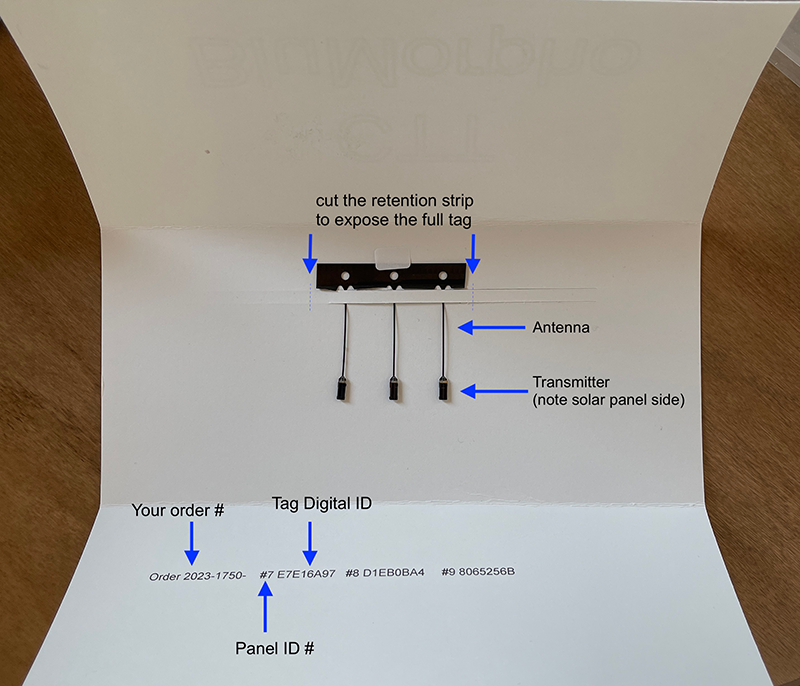
\includegraphics[width=0.5\textwidth,height=\textheight]{/Users/davidlapuma/Library/CloudStorage/Dropbox/CTT_Git/ctt_documentation/images/IMG_1557.png}
\caption{\emph{Fig 1. The tri-fold envelope holding your BlūMorpho tags.
Note the retention strip holding the antennas down, and the small white
sticker holding the panel strip to the envelope.}}\label{id}
}
\end{figure}

\begin{itemize}
\tightlist
\item
  \textbf{Note the tags are solar-panel up (also depicted in Fig 2)
  which is the way you will want to deploy them on an animal. }
\end{itemize}

\begin{figure}
\hypertarget{id}{%
\centering
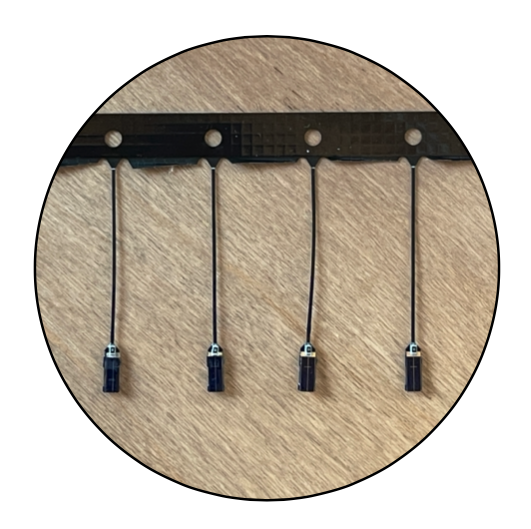
\includegraphics[width=0.45\textwidth,height=\textheight]{/Users/davidlapuma/Library/CloudStorage/Dropbox/CTT_Git/ctt_documentation/images/BluMorpho_SolarSide.png}
\caption{\emph{Fig 2. The upperside of the BlūMorpho transmitter showing
the solar panel as well as the small cutline indicating where you should
cut to separate the tag and antenna from the panel strip. This cut line
results in a 1/4 wavelength antenna.}}\label{id}
}
\end{figure}

\begin{itemize}
\tightlist
\item
  In Fig 2, also notice that there is a small white ``cut line'' at the
  top of the antenna, where it meets the panel strip. This is the ONLY
  place where you should cut your tag to remove it from the panel strip
  and deploy it on an animal.
\end{itemize}

\begin{figure}
\hypertarget{id}{%
\centering
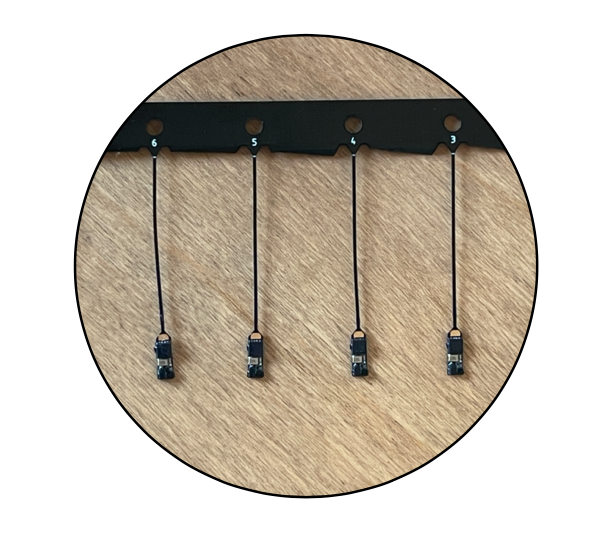
\includegraphics[width=0.5\textwidth,height=\textheight]{/Users/davidlapuma/Library/CloudStorage/Dropbox/CTT_Git/ctt_documentation/images/BluMorpho_ComponentSide.png}
\caption{\emph{Fig 3. The underside of the BlūMorpho tag showing the
reference ``Panel ID numbers'' along the top of the Panel}}\label{id}
}
\end{figure}

\begin{itemize}
\tightlist
\item
  In Fig 3 you'll see the same tags, but from the component side (the
  underside of the tag). Here you can see the Panel ID numbers on the
  panel strip. These numbers are your reference to the full Tag Digital
  ID \# that will show up on your receiver. Make sure you note these for
  your records, as the tag's ID is NOT printed on the tag itself.
\end{itemize}

\hypertarget{final-thoughts}{%
\section{Final Thoughts}\label{final-thoughts}}

This User Guide is a living document. Your experiences and input are
greatly appreciated so please don't hesitate to reach out to us
regarding what you'd like to see included here. You can submit your
suggestions and any errors to our \texttt{Customer\ Service\ Desk}
\href{https://celltracktech.com/pages/customer-service-desk-csd}{here}
and we will work to incorporate them in future revisions. All material ©
Cellular Tracking Technologies, 2023.

\end{document}
